\subsection{Definitions and Effects}
\label{subsec:ac-basics2}

Let's dive into the fascinating world of electromagnetic waves! These waves are the backbone of radio technology, and understanding their properties is crucial. At their core, electromagnetic waves are composed of two primary components: the electric field and the magnetic field. These fields are perpendicular to each other and to the direction of wave propagation. Imagine them as two dancers moving in perfect harmony, each influencing the other. 

Maxwell's equations describe four fundamental relationships in electromagnetism (and they're like the superhero team of physics - each one has its own special power!):
\begin{itemize}[noitemsep]    \item How electric charges create electric fields (Captain Electric's origin story)
    \item How magnetic fields are created by moving charges and changing electric fields (The Magnetic Marvel's secret technique)
    \item How magnetic fields circulate around electric currents and changing electric fields (The Dynamic Duo's team-up move)
    \item How magnetic poles always come in pairs - nature's way of saying "you complete me" (no lonely magnetic monopoles allowed!)
\end{itemize}

Now, let's talk about polarization. Polarization refers to the orientation of the electric field as the wave travels. If the electric field oscillates in a single plane, the wave is said to be linearly polarized. If the electric field rotates as the wave propagates, it can be circularly or elliptically polarized. The orientation of the electric field determines the polarization state, which is crucial for applications like satellite communication and radar systems.

\begin{figure}[h]
    \centering
    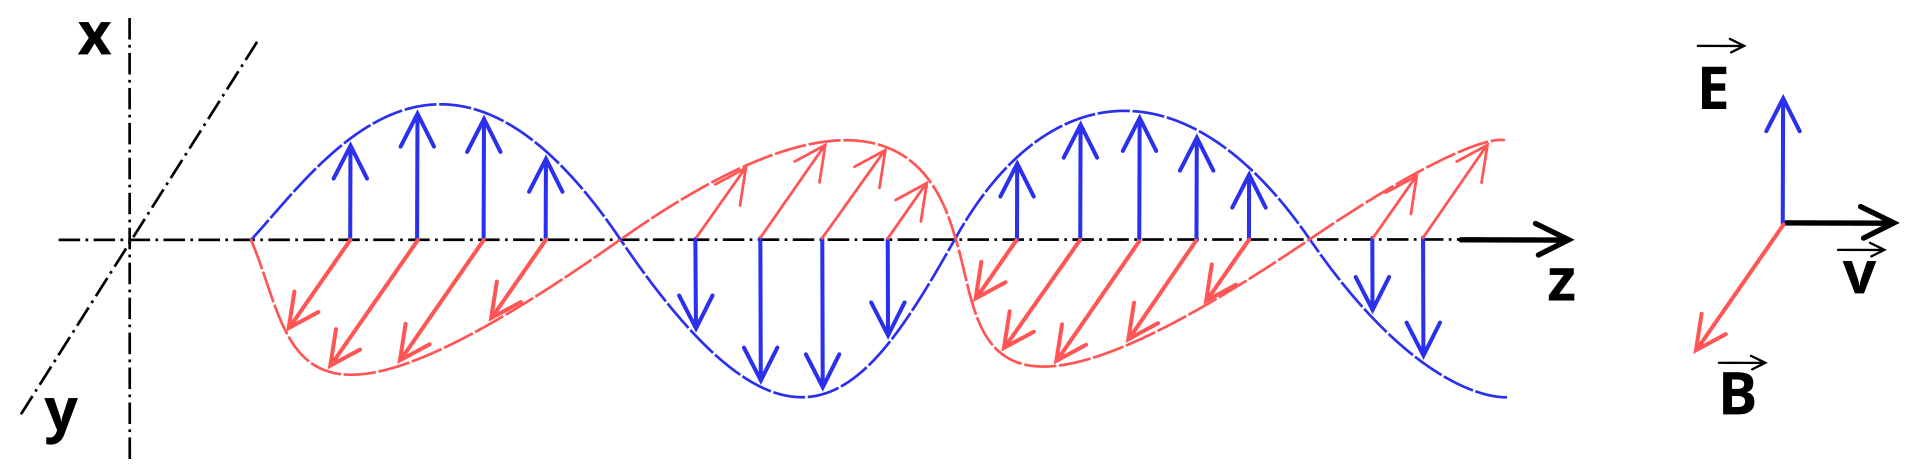
\includegraphics[width=0.8\textwidth]{tech/images/em-wave.png}
    \caption{Relationship between electric and magnetic fields in an electromagnetic wave. The electric field (E) and magnetic field (B) are perpendicular to each other and to the direction of wave propagation. As one field increases, the other follows 90 degrees later in space (like a synchronized dance where one partner bows while the other steps sideways). The wave's energy alternates between electric and magnetic fields as it travels through space, with both fields reaching their maximum and minimum values at different points.}
    \label{fig:em-wave}
    % Image prompt: Diagram showing the relationship between electric and magnetic fields in an electromagnetic wave. The electric field (E) and magnetic field (B) should be shown as perpendicular vectors, with the wave propagating in a direction perpendicular to both.
\end{figure}

\begin{figure}[h]
    \centering
    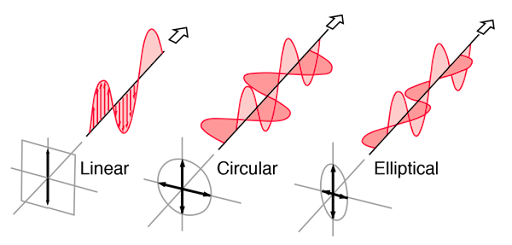
\includegraphics[width=0.8\textwidth]{tech/images/polarization.png}
    \caption{Radio wave polarization determined by the orientation of the electric field. Linear polarization occurs when the electric field oscillates in a single fixed plane (like a jump rope moving up and down). Circular polarization happens when the electric field rotates uniformly around the direction of propagation (like a spiral staircase). Elliptical polarization is similar to circular, but the field strength varies during rotation (imagine squishing that spiral staircase slightly).}
    \label{fig:polarization}
    % Image prompt: Illustration of radio wave polarization showing the orientation of the electric field. The electric field should be shown oscillating in different planes for linear, circular, and elliptical polarization.
\end{figure}

In summary, the electric and magnetic fields are the yin and yang of electromagnetic waves. They work together to create the waves that carry information across vast distances. Understanding their relationship and the concept of polarization is essential for anyone working in radio technology. So, next time you tune into your favorite radio station, remember the intricate dance of electric and magnetic fields that makes it all possible!

\begin{table}[h]
    \centering
    \begin{tabular}{|c|c|c|}
        \hline
        \textbf{Band} & \textbf{Frequency Range} & \textbf{Wavelength Range} \\
        \hline
        HF & 3 MHz to 30 MHz & 100 m to 10 m \\
        VHF & 30 MHz to 300 MHz & 10 m to 1 m \\
        UHF & 300 MHz to 3 GHz & 1 m to 10 cm \\
        SHF & 3 GHz to 30 GHz & 10 cm to 1 cm \\
        EHF & 30 GHz to 300 GHz & 1 cm to 1 mm \\
        \hline
    \end{tabular}
    \caption{Frequency and wavelength ranges for radio frequency bands.}
    \label{tab:frequency-ranges}
\end{table}
